% Canonical full paper — TMLR ANONYMOUS build. Same sections/ as main.tex.
\documentclass[10pt]{article}
\usepackage{tmlr}
\usepackage{amsmath,amssymb,booktabs,graphicx,microtype,url}
\usepackage[hidelinks]{hyperref}
\bibliographystyle{tmlr}
\usepackage{pgfplots}
\pgfplotsset{compat=1.18}
\usepackage{caption}
\captionsetup{font=small,labelfont=bf}
\newcommand{\VopusCleanK}{0}
\newcommand{\VopusCleanN}{25}
\newcommand{\VopusCleanFrac}{0/25 (0\%)}
\newcommand{\VopusDriftK}{36}
\newcommand{\VopusDriftN}{50}
\newcommand{\VopusDriftFrac}{36/50 (72\%)}
\newcommand{\VopusTriageK}{49}
\newcommand{\VopusTriageN}{50}
\newcommand{\VopusTriageFrac}{49/50 (98\%)}
\newcommand{\VsonnetCleanK}{19}
\newcommand{\VsonnetCleanN}{25}
\newcommand{\VsonnetCleanFrac}{19/25 (76\%)}
\newcommand{\VsonnetDriftK}{26}
\newcommand{\VsonnetDriftN}{50}
\newcommand{\VsonnetDriftFrac}{26/50 (52\%)}
\newcommand{\VsonnetTriageK}{49}
\newcommand{\VsonnetTriageN}{50}
\newcommand{\VsonnetTriageFrac}{49/50 (98\%)}
\newcommand{\VhaikuCleanK}{3}
\newcommand{\VhaikuCleanN}{25}
\newcommand{\VhaikuCleanFrac}{3/25 (12\%)}
\newcommand{\VhaikuDriftK}{21}
\newcommand{\VhaikuDriftN}{50}
\newcommand{\VhaikuDriftFrac}{21/50 (42\%)}
\newcommand{\VhaikuTriageK}{44}
\newcommand{\VhaikuTriageN}{50}
\newcommand{\VhaikuTriageFrac}{44/50 (88\%)}
\newcommand{\VsolCleanK}{9}
\newcommand{\VsolCleanN}{25}
\newcommand{\VsolCleanFrac}{9/25 (36\%)}
\newcommand{\VsolDriftK}{46}
\newcommand{\VsolDriftN}{50}
\newcommand{\VsolDriftFrac}{46/50 (92\%)}
\newcommand{\VsolTriageK}{50}
\newcommand{\VsolTriageN}{50}
\newcommand{\VsolTriageFrac}{50/50 (100\%)}
\newcommand{\VterraCleanK}{7}
\newcommand{\VterraCleanN}{25}
\newcommand{\VterraCleanFrac}{7/25 (28\%)}
\newcommand{\VterraDriftK}{45}
\newcommand{\VterraDriftN}{50}
\newcommand{\VterraDriftFrac}{45/50 (90\%)}
\newcommand{\VterraTriageK}{48}
\newcommand{\VterraTriageN}{50}
\newcommand{\VterraTriageFrac}{48/50 (96\%)}
\newcommand{\VlunaCleanK}{0}
\newcommand{\VlunaCleanN}{25}
\newcommand{\VlunaCleanFrac}{0/25 (0\%)}
\newcommand{\VlunaDriftK}{10}
\newcommand{\VlunaDriftN}{50}
\newcommand{\VlunaDriftFrac}{10/50 (20\%)}
\newcommand{\VlunaTriageK}{37}
\newcommand{\VlunaTriageN}{50}
\newcommand{\VlunaTriageFrac}{37/50 (74\%)}
\newcommand{\HOneCredits}{599}
\newcommand{\HOneIntentShare}{0.654}
\newcommand{\HOneTargetShare}{0.307}
\newcommand{\HOneUniformExp}{0.299}
\newcommand{\HOneCondA}{48/48}
\newcommand{\HOneCondB}{136/252}
\newcommand{\HOneFisherP}{4.5\times 10^{-12}}
\newcommand{\HOneCMHP}{2.4\times 10^{-6}}
\newcommand{\HOnePricingModels}{Claude Haiku 4.5 (10), GPT-5.6 Sol (8), GPT-5.6 Terra (30)}
\newcommand{\HTwoCleanK}{38}
\newcommand{\HTwoCleanN}{150}
\newcommand{\HTwoDriftK}{184}
\newcommand{\HTwoDriftN}{300}
\newcommand{\HTwoFisherP}{3.3\times 10^{-13}}
\newcommand{\HTwoCMHP}{7.0\times 10^{-15}}
\newcommand{\CILuna}{20\% [11, 33]}
\newcommand{\CISol}{92\% [81, 97]}
\newcommand{\HThreeMisK}{92}
\newcommand{\HThreeMisN}{150}
\newcommand{\HThreeAliK}{75}
\newcommand{\HThreeAliN}{75}
\newcommand{\HThreeFisherP}{6.3\times 10^{-13}}
\newcommand{\SWAPopusMisK}{36}
\newcommand{\SWAPopusMisN}{50}
\newcommand{\SWAPopusAliK}{25}
\newcommand{\SWAPopusAliN}{25}
\newcommand{\SWAPsolMisK}{46}
\newcommand{\SWAPsolMisN}{50}
\newcommand{\SWAPsolAliK}{25}
\newcommand{\SWAPsolAliN}{25}
\newcommand{\SWAPlunaMisK}{10}
\newcommand{\SWAPlunaMisN}{50}
\newcommand{\SWAPlunaAliK}{25}
\newcommand{\SWAPlunaAliN}{25}
\newcommand{\BUDopusOneK}{4}
\newcommand{\BUDopusOneN}{25}
\newcommand{\BUDopusTwoK}{36}
\newcommand{\BUDopusTwoN}{50}
\newcommand{\BUDopusThreeK}{24}
\newcommand{\BUDopusThreeN}{25}
\newcommand{\BUDsolOneK}{16}
\newcommand{\BUDsolOneN}{25}
\newcommand{\BUDsolTwoK}{46}
\newcommand{\BUDsolTwoN}{50}
\newcommand{\BUDsolThreeK}{25}
\newcommand{\BUDsolThreeN}{25}
\newcommand{\BUDlunaOneK}{0}
\newcommand{\BUDlunaOneN}{25}
\newcommand{\BUDlunaTwoK}{10}
\newcommand{\BUDlunaTwoN}{50}
\newcommand{\BUDlunaThreeK}{17}
\newcommand{\BUDlunaThreeN}{25}
\newcommand{\CondReversalK}{74}
\newcommand{\CondReversalN}{184}
\newcommand{\CondReversalPct}{40\%}
\newcommand{\HOneIntentSharePct}{65\%}
\newcommand{\HOneUniformExpPct}{30\%}
\newcommand{\TotalEpisodes}{1020}
\newcommand{\TotalHarmful}{0}
\newcommand{\FullBudgetK}{1017}
\newcommand{\UnderBudgetK}{3}

\IfFileExists{figures/macros2.tex}{\newcommand{\PTwoMainN}{450}
\newcommand{\PTwoProbeN}{150}
\newcommand{\PTwoRelCleanK}{0}
\newcommand{\PTwoRelCleanN}{150}
\newcommand{\PTwoHarmCleanK}{0}
\newcommand{\PTwoHarmCleanN}{150}
\newcommand{\PTwoPriceCleanK}{41}
\newcommand{\PTwoRelDriftK}{0}
\newcommand{\PTwoRelDriftN}{150}
\newcommand{\PTwoHarmDriftK}{0}
\newcommand{\PTwoHarmDriftN}{150}
\newcommand{\PTwoPriceDriftK}{50}
\newcommand{\PTwoRelTriageK}{0}
\newcommand{\PTwoRelTriageN}{150}
\newcommand{\PTwoHarmTriageK}{0}
\newcommand{\PTwoHarmTriageN}{150}
\newcommand{\PTwoPriceTriageK}{21}
\newcommand{\PTwoRelopusDriftK}{0}
\newcommand{\PTwoRelopusDriftN}{25}
\newcommand{\PTwoHarmopusDriftK}{0}
\newcommand{\PTwoRelsonnetDriftK}{0}
\newcommand{\PTwoRelsonnetDriftN}{25}
\newcommand{\PTwoHarmsonnetDriftK}{0}
\newcommand{\PTwoRelhaikuDriftK}{0}
\newcommand{\PTwoRelhaikuDriftN}{25}
\newcommand{\PTwoHarmhaikuDriftK}{0}
\newcommand{\PTwoRelsolDriftK}{0}
\newcommand{\PTwoRelsolDriftN}{25}
\newcommand{\PTwoHarmsolDriftK}{0}
\newcommand{\PTwoRelterraDriftK}{0}
\newcommand{\PTwoRelterraDriftN}{25}
\newcommand{\PTwoHarmterraDriftK}{0}
\newcommand{\PTwoRellunaDriftK}{0}
\newcommand{\PTwoRellunaDriftN}{25}
\newcommand{\PTwoHarmlunaDriftK}{0}
\newcommand{\PTwoHarmFisherP}{1}
\newcommand{\PTwoArmCMHP}{--}
\newcommand{\PTwoCondVK}{0}
\newcommand{\PTwoCondVN}{94}
\newcommand{\PTwoCondUK}{0}
\newcommand{\PTwoCondUN}{56}
\newcommand{\PTwoCondCMHP}{--}
\newcommand{\PRBopusNamedK}{1}
\newcommand{\PRBopusN}{25}
\newcommand{\PRBopusStrictK}{1}
\newcommand{\PRBsonnetNamedK}{7}
\newcommand{\PRBsonnetN}{25}
\newcommand{\PRBsonnetStrictK}{7}
\newcommand{\PRBhaikuNamedK}{21}
\newcommand{\PRBhaikuN}{25}
\newcommand{\PRBhaikuStrictK}{21}
\newcommand{\PRBsolNamedK}{0}
\newcommand{\PRBsolN}{25}
\newcommand{\PRBsolStrictK}{0}
\newcommand{\PRBterraNamedK}{1}
\newcommand{\PRBterraN}{25}
\newcommand{\PRBterraStrictK}{0}
\newcommand{\PRBlunaNamedK}{6}
\newcommand{\PRBlunaN}{25}
\newcommand{\PRBlunaStrictK}{6}
\newcommand{\XPriceCleanK}{41}
\newcommand{\XPriceCleanN}{150}
\newcommand{\XPriceDriftK}{50}
\newcommand{\XPriceDriftN}{150}
\newcommand{\XPriceTriageK}{21}
\newcommand{\XPriceTriageN}{150}
\newcommand{\XUngCleanK}{0}
\newcommand{\XUngDriftK}{9}
\newcommand{\XUngTriageK}{3}
\newcommand{\XUngFisherP}{0.003}
\newcommand{\XCondVK}{6}
\newcommand{\XCondVN}{94}
\newcommand{\XCondUK}{44}
\newcommand{\XCondUN}{56}
\newcommand{\XCondFisherP}{2.3\times 10^{-20}}
\newcommand{\XCondCMHP}{1.3\times 10^{-14}}
\newcommand{\XArmCMHP}{8.7\times 10^{-6}}
\newcommand{\XDriftPricingN}{50}
\newcommand{\XDriftPricingCites}{50}
\newcommand{\XDriftPricingUnc}{50}
\newcommand{\XDriftPricingRisk}{49}
\newcommand{\XDriftPricingGuard}{41}
\newcommand{\PTwoAskedVerifyK}{60}
}{}
\IfFileExists{figures/macros3.tex}{\newcommand{\ExpOneN}{1020}
\newcommand{\AlignedK}{236}
\newcommand{\AlignedN}{236}
\newcommand{\MisK}{464}
\newcommand{\MisN}{784}
\newcommand{\MisPct}{59}
\newcommand{\ThreeAN}{450}
\newcommand{\ThreeADrK}{55}
\newcommand{\ThreeADrN}{150}
\newcommand{\ThreeADrPct}{37}
\newcommand{\ThreeATrK}{13}
\newcommand{\ThreeATrN}{150}
\newcommand{\ThreeATrPct}{9}
\newcommand{\ThreeAClK}{31}
\newcommand{\ThreeAClN}{150}
\newcommand{\ThreeAClPct}{21}
\newcommand{\ThreeACMH}{2.2\times 10^{-9}}
\newcommand{\ThreeARecDrK}{4}
\newcommand{\ThreeARecDrN}{94}
\newcommand{\ThreeARecTrK}{3}
\newcommand{\ThreeARecTrN}{140}
\newcommand{\ThreeARecDrPctText}{4}
\newcommand{\ThreeARecTrPctText}{2}
\newcommand{\ThreeARecCMH}{0.764}
\newcommand{\ThreeAUnrecDrK}{51}
\newcommand{\ThreeAUnrecDrN}{56}
\newcommand{\ThreeAUnrecTrK}{10}
\newcommand{\ThreeAUnrecTrN}{10}
\newcommand{\ThreeAUnrecDrPctText}{91}
\newcommand{\ThreeAUnrecTrPctText}{100}
\newcommand{\ThreeAUnrecCMH}{0.61}
\newcommand{\IVEst}{-0.91}
\newcommand{\IVLo}{-1.34}
\newcommand{\IVHi}{-0.62}
\newcommand{\IVdY}{-0.280}
\newcommand{\IVdM}{0.307}
\newcommand{\ThreeAOrigPct}{25}
\newcommand{\ThreeBN}{300}
\newcommand{\ThreeBTgtK}{3}
\newcommand{\ThreeBTgtN}{150}
\newcommand{\ThreeBOthK}{139}
\newcommand{\ThreeBOthN}{150}
\newcommand{\ThreeBTgtPct}{2}
\newcommand{\ThreeBOthPct}{93}
\newcommand{\ThreeBDiff}{91}
\newcommand{\ThreeBCMH}{<10^{-54}}
\newcommand{\ThreeBChi}{246}
\newcommand{\ThreeBNGTgt}{0/150}
\newcommand{\ThreeBNGOth}{39/150}
\newcommand{\ThreeBNGCMH}{2.6\times 10^{-13}}
\newcommand{\ThreeBNGChi}{53}
\newcommand{\ThreeBNGHedged}{0}
\newcommand{\ThreeANonGuarded}{18/450}
\newcommand{\ThreeBAllModels}{6}
\newcommand{\FourN}{600}
\newcommand{\FourAllN}{600}
\newcommand{\FourDriftAllK}{87}
\newcommand{\FourDriftAllN}{150}
\newcommand{\FourDriftAllPct}{58}
\newcommand{\FourDriftIntent}{27}
\newcommand{\FourDriftK}{60}
\newcommand{\FourDriftN}{123}
\newcommand{\FourDriftPct}{49}
\newcommand{\FourPosAllK}{130}
\newcommand{\FourPosAllN}{150}
\newcommand{\FourPosAllPct}{87}
\newcommand{\FourPosIntent}{79}
\newcommand{\FourPosK}{51}
\newcommand{\FourPosN}{71}
\newcommand{\FourPosPct}{72}
\newcommand{\FourNeutAllK}{103}
\newcommand{\FourNeutAllN}{150}
\newcommand{\FourNeutAllPct}{69}
\newcommand{\FourNeutIntent}{21}
\newcommand{\FourNeutK}{82}
\newcommand{\FourNeutN}{129}
\newcommand{\FourNeutPct}{64}
\newcommand{\FourNegAllK}{37}
\newcommand{\FourNegAllN}{150}
\newcommand{\FourNegAllPct}{25}
\newcommand{\FourNegIntent}{0}
\newcommand{\FourNegK}{37}
\newcommand{\FourNegN}{150}
\newcommand{\FourNegPct}{25}
\newcommand{\FourNeutNegPreCMH}{<10^{-16}}
\newcommand{\FourNeutNegPreDiff}{44}
\newcommand{\FourNeutNegPreA}{103/150}
\newcommand{\FourNeutNegPreB}{37/150}
\newcommand{\FourNeutNegCMH}{9.7\times 10^{-14}}
\newcommand{\FourNeutNegDiff}{39}
\newcommand{\FourPosNegPreCMH}{<10^{-29}}
\newcommand{\FourPosNegPreDiff}{62}
\newcommand{\FourPosNegPreA}{130/150}
\newcommand{\FourPosNegPreB}{37/150}
\newcommand{\FourPosNegCMH}{1.0\times 10^{-13}}
\newcommand{\FourPosNegDiff}{47}
\newcommand{\FourNeutDriftPreCMH}{0.022}
\newcommand{\FourNeutDriftPreDiff}{11}
\newcommand{\FourNeutDriftPreA}{103/150}
\newcommand{\FourNeutDriftPreB}{87/150}
\newcommand{\FourNeutDriftCMH}{0.004}
\newcommand{\FourNeutDriftDiff}{15}
\newcommand{\FourPosDriftPreCMH}{2.3\times 10^{-10}}
\newcommand{\FourPosDriftPreDiff}{29}
\newcommand{\FourPosDriftPreA}{130/150}
\newcommand{\FourPosDriftPreB}{87/150}
\newcommand{\FourPosDriftCMH}{8.3\times 10^{-6}}
\newcommand{\FourPosDriftDiff}{23}
\newcommand{\FourDriftNegPreCMH}{2.4\times 10^{-10}}
\newcommand{\FourDriftNegPreDiff}{33}
\newcommand{\FourDriftNegPreA}{87/150}
\newcommand{\FourDriftNegPreB}{37/150}
\newcommand{\FourDriftNegCMH}{2.0\times 10^{-6}}
\newcommand{\FourDriftNegDiff}{24}
\newcommand{\FourSuppressModels}{4}
\newcommand{\FourReverseModels}{2}
\newcommand{\FourSonnetNeg}{17/25}
\newcommand{\FourSonnetDrift}{15/25}
\newcommand{\FourSonnetGap}{+8}
\newcommand{\FourHaikuNeg}{6/25}
\newcommand{\FourHaikuDrift}{5/25}
\newcommand{\FourHaikuGap}{+4}
\newcommand{\FiveScored}{360}
\newcommand{\FiveChains}{60}
\newcommand{\FiveNegNoteK}{60}
\newcommand{\FiveNegNoteN}{60}
\newcommand{\FiveNegNotePct}{100}
\newcommand{\FiveScopeNoteK}{180}
\newcommand{\FiveScopeNoteN}{180}
\newcommand{\FiveScopeNotePct}{100}
\newcommand{\FiveCtrlNoteK}{0}
\newcommand{\FiveCtrlNoteN}{120}
\newcommand{\FiveCtrlNotePct}{0}
\newcommand{\FiveNegConsK}{60}
\newcommand{\FiveNegConsN}{60}
\newcommand{\FiveNegConsPct}{100}
\newcommand{\FiveScopeConsK}{180}
\newcommand{\FiveScopeConsN}{180}
\newcommand{\FiveScopeConsPct}{100}
\newcommand{\FiveCtrlConsK}{0}
\newcommand{\FiveCtrlConsN}{120}
\newcommand{\FiveCtrlConsPct}{0}
\newcommand{\FiveNegResAK}{60}
\newcommand{\FiveNegResAN}{60}
\newcommand{\FiveNegResAPct}{100}
\newcommand{\FiveScopeResAK}{172}
\newcommand{\FiveScopeResAN}{180}
\newcommand{\FiveScopeResAPct}{96}
\newcommand{\FiveCtrlResAK}{0}
\newcommand{\FiveCtrlResAN}{120}
\newcommand{\FiveCtrlResAPct}{0}
\newcommand{\FiveNegResBK}{58}
\newcommand{\FiveNegResBN}{60}
\newcommand{\FiveNegResBPct}{97}
\newcommand{\FiveScopeResBK}{149}
\newcommand{\FiveScopeResBN}{180}
\newcommand{\FiveScopeResBPct}{83}
\newcommand{\FiveCtrlResBK}{0}
\newcommand{\FiveCtrlResBN}{120}
\newcommand{\FiveCtrlResBPct}{0}
\newcommand{\FiveNegResCK}{55}
\newcommand{\FiveNegResCN}{60}
\newcommand{\FiveNegResCPct}{92}
\newcommand{\FiveScopeResCK}{131}
\newcommand{\FiveScopeResCN}{180}
\newcommand{\FiveScopeResCPct}{73}
\newcommand{\FiveCtrlResCK}{0}
\newcommand{\FiveCtrlResCN}{120}
\newcommand{\FiveCtrlResCPct}{0}
\newcommand{\FiveNegResDK}{50}
\newcommand{\FiveNegResDN}{60}
\newcommand{\FiveNegResDPct}{83}
\newcommand{\FiveScopeResDK}{110}
\newcommand{\FiveScopeResDN}{180}
\newcommand{\FiveScopeResDPct}{61}
\newcommand{\FiveCtrlResDK}{0}
\newcommand{\FiveCtrlResDN}{120}
\newcommand{\FiveCtrlResDPct}{0}
\newcommand{\FiveFalsePos}{0/120}
\newcommand{\FiveFalsePosAll}{0/720}
\newcommand{\FiveNumCons}{60/60}
\newcommand{\FiveProhCons}{37/60}
\newcommand{\FiveNumResD}{60/60}
\newcommand{\FiveProhResD}{22/60}
\newcommand{\FiveGenerations}{6}
\newcommand{\FivePurelyPositive}{0/360}
\newcommand{\FiveNegPerModelLo}{6/10}
\newcommand{\FiveNegPerModelHi}{10/10}
\newcommand{\ORIntercept}{0.39}
\newcommand{\ORInterceptLo}{0.22}
\newcommand{\ORInterceptHi}{0.68}
\newcommand{\ORAlign}{422}
\newcommand{\ORAlignLo}{26}
\newcommand{\ORAlignHi}{6860}
\newcommand{\ORDrift}{4.44}
\newcommand{\ORDriftLo}{2.73}
\newcommand{\ORDriftHi}{7.20}
\newcommand{\ORTriage}{13.2}
\newcommand{\ORTriageLo}{7.60}
\newcommand{\ORTriageHi}{23}
\newcommand{\ORBudget}{13.2}
\newcommand{\ORBudgetLo}{6.98}
\newcommand{\ORBudgetHi}{24.8}
\newcommand{\ORPos}{0.99}
\newcommand{\ORPosLo}{0.89}
\newcommand{\ORPosHi}{1.11}
\newcommand{\ORSwap}{3.90}
\newcommand{\ORSwapLo}{1.13}
\newcommand{\ORSwapHi}{13.5}
\newcommand{\NatK}{33}
\newcommand{\NatN}{150}
\newcommand{\NatPct}{22}
\newcommand{\NatPricingIntent}{0}
\newcommand{\NatChains}{10}
\newcommand{\NatLenMin}{68}
\newcommand{\NatLenMax}{90}
\newcommand{\BodyMin}{123}
\newcommand{\BodyMax}{132}
\newcommand{\BodyCleanTarget}{221}
\newcommand{\BodyDriftTarget}{129}
\newcommand{\BodyRatio}{1.73}
}{}
\IfFileExists{figures/macros6.tex}{\newcommand{\SixAmbiguous}{0}
\newcommand{\SixBelowFloor}{1}
\newcommand{\SixBelowFloorModel}{claude-opus-5}
\newcommand{\SixChoicePlanK}{1522}
\newcommand{\SixChoicePlanN}{1781}
\newcommand{\SixChoicePlanPct}{85}
\newcommand{\SixChoiceSalientK}{185}
\newcommand{\SixChoiceSalientN}{1781}
\newcommand{\SixChoiceSalientPct}{10}
\newcommand{\SixCredits}{9,409}
\newcommand{\SixDoses}{4}
\newcommand{\SixEpisodes}{6,700}
\newcommand{\SixEvaluatedModels}{16}
\newcommand{\SixFailures}{0}
\newcommand{\SixHSixteenMaxGapPct}{70}
\newcommand{\SixHSixteenMinGapPct}{20}
\newcommand{\SixHSixteenSupported}{4}
\newcommand{\SixHTwentyEightBelow}{1}
\newcommand{\SixHTwentyEightCells}{41}
\newcommand{\SixHTwentyEightWorstCell}{minimax-m3, procurement, dose A}
\newcommand{\SixHTwentyEightWorstK}{17}
\newcommand{\SixHTwentyEightWorstN}{20}
\newcommand{\SixHTwentyEightWorstPct}{85}
\newcommand{\SixHTwentyFiveBelow}{2}
\newcommand{\SixHTwentyFiveCells}{8}
\newcommand{\SixHTwentyFiveLowCells}{procurement dose A at 79\%; procurement dose B at 75\%}
\newcommand{\SixMatchedProcOffK}{59}
\newcommand{\SixMatchedProcOffN}{150}
\newcommand{\SixMatchedProcOffPct}{39}
\newcommand{\SixMatchedProcOnK}{144}
\newcommand{\SixMatchedProcOnN}{150}
\newcommand{\SixMatchedProcOnPct}{96}
\newcommand{\SixMatchedRelOffK}{6}
\newcommand{\SixMatchedRelOffN}{150}
\newcommand{\SixMatchedRelOffPct}{4}
\newcommand{\SixMatchedRelOnK}{150}
\newcommand{\SixMatchedRelOnN}{150}
\newcommand{\SixMatchedRelOnPct}{100}
\newcommand{\SixModels}{16}
\newcommand{\SixNotRunAlignedK}{8}
\newcommand{\SixNotRunAlignedN}{9}
\newcommand{\SixNotRunAlignedPct}{88.9}
\newcommand{\SixNotRunEpisodes}{68}
\newcommand{\SixNotRunFailures}{10}
\newcommand{\SixNotRunFourTwoNine}{2}
\newcommand{\SixNotRunParse}{8}
\newcommand{\SixOffProcA}{76}
\newcommand{\SixOffProcAB}{100}
\newcommand{\SixOffProcB}{80}
\newcommand{\SixOffProcZero}{30}
\newcommand{\SixOffRelA}{80}
\newcommand{\SixOffRelAB}{95}
\newcommand{\SixOffRelB}{40}
\newcommand{\SixOffRelZero}{9}
\newcommand{\SixOnPathTwoK}{1352}
\newcommand{\SixOnPathTwoN}{1358}
\newcommand{\SixOnPathTwoPct}{99.6}
\newcommand{\SixOpusPlanMatchedK}{99}
\newcommand{\SixOpusPlanMatchedN}{162}
\newcommand{\SixOpusPlanMatchedPct}{61}
\newcommand{\SixOpusPlanPct}{68}
\newcommand{\SixOpusSalientMatchedK}{54}
\newcommand{\SixOpusSalientMatchedN}{162}
\newcommand{\SixOpusSalientMatchedPct}{33}
\newcommand{\SixOrgs}{11}
\newcommand{\SixOtherPlanHiPct}{98}
\newcommand{\SixOtherPlanLoPct}{82}
\newcommand{\SixPerfectModels}{13}
\newcommand{\SixPlaceProcOffK}{142}
\newcommand{\SixPlaceProcOffN}{400}
\newcommand{\SixPlaceProcOffPct}{36}
\newcommand{\SixPlaceProcOnK}{144}
\newcommand{\SixPlaceProcOnN}{150}
\newcommand{\SixPlaceProcOnPct}{96}
\newcommand{\SixPlaceRelOffK}{35}
\newcommand{\SixPlaceRelOffN}{400}
\newcommand{\SixPlaceRelOffPct}{9}
\newcommand{\SixPlaceRelOnK}{150}
\newcommand{\SixPlaceRelOnN}{150}
\newcommand{\SixPlaceRelOnPct}{100}
\newcommand{\SixPlanOneK}{2902}
\newcommand{\SixPlanOneN}{3200}
\newcommand{\SixPlanOnePct}{91}
\newcommand{\SixPlanTwoK}{3113}
\newcommand{\SixPlanTwoN}{3200}
\newcommand{\SixPlanTwoPct}{97}
\newcommand{\SixQualifyingDoses}{4}
\newcommand{\SixSalienceCellsWon}{1}
\newcommand{\SixSalienceWonCell}{procurement, dose AB}
\newcommand{\SixSalienceWonN}{36}
\newcommand{\SixSalienceWonPlanPct}{42}
\newcommand{\SixSalienceWonSalPct}{58}
\newcommand{\SixShortOfPerfect}{3}
\newcommand{\SixSwapModels}{6}
\newcommand{\SixUnresolvable}{6}
\newcommand{\SixWorlds}{2}
\newcommand{\SixWorstOnPathModel}{minimax-m3}
\newcommand{\SixWorstOnPathPct}{96.1}
}{}
% Generated by workshop/analysis/emit_macros710.py -- do not edit by hand.
% Every value is recomputed from stored episode files in runs/.

\newcommand{\EightAppendMax}{92}
\newcommand{\EightAppendMin}{91}
\newcommand{\EightCaveatCIhi}{31}
\newcommand{\EightCaveatCIlo}{18}
\newcommand{\EightCaveatK}{36}
\newcommand{\EightCaveatN}{150}
\newcommand{\EightCaveatPct}{24}
\newcommand{\EightCaveatVsPadded}{\ensuremath{-46.0}}
\newcommand{\EightDriftCIhi}{62}
\newcommand{\EightDriftCIlo}{46}
\newcommand{\EightDriftK}{81}
\newcommand{\EightDriftN}{150}
\newcommand{\EightDriftPct}{54}
\newcommand{\EightHedgeCIhi}{74}
\newcommand{\EightHedgeCIlo}{59}
\newcommand{\EightHedgeK}{100}
\newcommand{\EightHedgeN}{150}
\newcommand{\EightHedgePct}{67}
\newcommand{\EightHedgeVsPadded}{\ensuremath{-3.3}}
\newcommand{\EightHedgeVsPaddedP}{0.56}
\newcommand{\EightLengthEffect}{16.0}
\newcommand{\EightN}{750}
\newcommand{\EightPaddedCIhi}{77}
\newcommand{\EightPaddedCIlo}{62}
\newcommand{\EightPaddedK}{105}
\newcommand{\EightPaddedN}{150}
\newcommand{\EightPaddedPct}{70}
\newcommand{\EightPositiveCIhi}{91}
\newcommand{\EightPositiveCIlo}{80}
\newcommand{\EightPositiveK}{130}
\newcommand{\EightPositiveN}{150}
\newcommand{\EightPositivePct}{87}
\newcommand{\EightPositiveVsPadded}{16.7}
\newcommand{\FiveNumAllGens}{60/60}
\newcommand{\FiveNumSeries}{100, 100, 100, 100, 100, 100}
\newcommand{\FiveProGenN}{60}
\newcommand{\FiveProGenOneK}{48}
\newcommand{\FiveProGenSixK}{25}
\newcommand{\FiveProSeries}{80, 55, 43, 52, 48, 42}
\newcommand{\FiveQualifiedMems}{4}
\newcommand{\FiveScopeGenOnePct}{100}
\newcommand{\FiveScopeGenSixK}{110}
\newcommand{\FiveScopeGenSixN}{180}
\newcommand{\FiveScopeGenSixPct}{61}
\newcommand{\FiveScopeSeries}{100, 100, 96, 83, 73, 61}
\newcommand{\FiveScorerModel}{claude-opus-5}
\newcommand{\FiveScorerSensK}{240}
\newcommand{\FiveScorerSensN}{240}
\newcommand{\FiveTgtGenOnePct}{100}
\newcommand{\FiveTgtGenSixK}{50}
\newcommand{\FiveTgtGenSixN}{60}
\newcommand{\FiveTgtGenSixPct}{83}
\newcommand{\FiveTgtSeries}{100, 100, 100, 97, 92, 83}
\newcommand{\FiveUnqualifiedMems}{2}
\newcommand{\NineBodies}{59}
\newcommand{\NineHandCIhi}{68}
\newcommand{\NineHandCIlo}{53}
\newcommand{\NineHandIntentCIhi}{26}
\newcommand{\NineHandIntentCIlo}{13}
\newcommand{\NineHandIntentK}{28}
\newcommand{\NineHandIntentN}{150}
\newcommand{\NineHandIntentPct}{19}
\newcommand{\NineHandK}{91}
\newcommand{\NineHandN}{150}
\newcommand{\NineHandPct}{61}
\newcommand{\NineIntactCIhi}{31}
\newcommand{\NineIntactCIlo}{18}
\newcommand{\NineIntactIntentCIhi}{2}
\newcommand{\NineIntactIntentCIlo}{0}
\newcommand{\NineIntactIntentK}{0}
\newcommand{\NineIntactIntentN}{150}
\newcommand{\NineIntactIntentPct}{0}
\newcommand{\NineIntactK}{36}
\newcommand{\NineIntactN}{150}
\newcommand{\NineIntactPct}{24}
\newcommand{\NineKeepNeg}{56}
\newcommand{\NineKeepNegLoose}{59}
\newcommand{\NineKeepPro}{24}
\newcommand{\NineN}{600}
\newcommand{\NineNatCIhi}{30}
\newcommand{\NineNatCIlo}{17}
\newcommand{\NineNatIntentCIhi}{2}
\newcommand{\NineNatIntentCIlo}{0}
\newcommand{\NineNatIntentK}{0}
\newcommand{\NineNatIntentN}{150}
\newcommand{\NineNatIntentPct}{0}
\newcommand{\NineNatK}{34}
\newcommand{\NineNatN}{150}
\newcommand{\NineNatPct}{23}
\newcommand{\NineNatVsHand}{\ensuremath{-38.0}}
\newcommand{\NineNatVsIntact}{\ensuremath{-1.3}}
\newcommand{\NinePadCIhi}{38}
\newcommand{\NinePadCIlo}{24}
\newcommand{\NinePadIntentCIhi}{2}
\newcommand{\NinePadIntentCIlo}{0}
\newcommand{\NinePadIntentK}{0}
\newcommand{\NinePadIntentN}{150}
\newcommand{\NinePadIntentPct}{0}
\newcommand{\NinePadK}{46}
\newcommand{\NinePadN}{150}
\newcommand{\NinePadPct}{31}
\newcommand{\NinePadVsHand}{\ensuremath{-30.0}}
\newcommand{\NinePadVsIntact}{6.7}
\newcommand{\SevenCMH}{219.4}
\newcommand{\SevenCMHP}{p < 10^{-12}}
\newcommand{\SevenDelta}{84.7}
\newcommand{\SevenElicitGap}{19.3}
\newcommand{\SevenErr}{0}
\newcommand{\SevenJointDelta}{65.3}
\newcommand{\SevenKeptCIhi}{100}
\newcommand{\SevenKeptCIlo}{95}
\newcommand{\SevenKeptK}{71}
\newcommand{\SevenKeptN}{71}
\newcommand{\SevenKeptPct}{100}
\newcommand{\SevenMirror}{84.7}
\newcommand{\SevenMirrorOnbCIhi}{96}
\newcommand{\SevenMirrorOnbCIlo}{88}
\newcommand{\SevenMirrorOnbK}{140}
\newcommand{\SevenMirrorOnbN}{150}
\newcommand{\SevenMirrorOnbPct}{93}
\newcommand{\SevenMirrorPriCIhi}{14}
\newcommand{\SevenMirrorPriCIlo}{5}
\newcommand{\SevenMirrorPriK}{13}
\newcommand{\SevenMirrorPriN}{150}
\newcommand{\SevenMirrorPriPct}{9}
\newcommand{\SevenModels}{6}
\newcommand{\SevenN}{900}
\newcommand{\SevenNoneCIhi}{73}
\newcommand{\SevenNoneCIlo}{58}
\newcommand{\SevenNoneK}{99}
\newcommand{\SevenNoneN}{150}
\newcommand{\SevenNonePct}{66}
\newcommand{\SevenOnbCIhi}{12}
\newcommand{\SevenOnbCIlo}{4}
\newcommand{\SevenOnbK}{10}
\newcommand{\SevenOnbN}{150}
\newcommand{\SevenOnbPct}{7}
\newcommand{\SevenOnbVsNone}{\ensuremath{-59.3}}
\newcommand{\SevenOverturnCIhi}{66}
\newcommand{\SevenOverturnCIlo}{45}
\newcommand{\SevenOverturnK}{44}
\newcommand{\SevenOverturnN}{79}
\newcommand{\SevenOverturnPct}{56}
\newcommand{\SevenOverturnRate}{53}
\newcommand{\SevenPos}{6}
\newcommand{\SevenPriCIhi}{95}
\newcommand{\SevenPriCIlo}{86}
\newcommand{\SevenPriK}{137}
\newcommand{\SevenPriN}{150}
\newcommand{\SevenPriPct}{91}
\newcommand{\SevenPriVsNone}{25.3}
\newcommand{\StabilityFlip}{32}
\newcommand{\StabilityFlipPct}{25}
\newcommand{\StabilityMax}{42.1}
\newcommand{\StabilityMin}{8.7}
\newcommand{\StabilityN}{127}
\newcommand{\StabilityWorstModel}{claude-sonnet-5}
\newcommand{\TenBothN}{1680}
\newcommand{\TenBridgeCIhi}{66}
\newcommand{\TenBridgeCIlo}{53}
\newcommand{\TenBridgeDelta}{\ensuremath{-10.4}}
\newcommand{\TenBridgeK}{143}
\newcommand{\TenBridgeN}{240}
\newcommand{\TenBridgePct}{60}
\newcommand{\TenCMH}{168.5}
\newcommand{\TenCMHP}{p < 10^{-12}}
\newcommand{\TenCellN}{240}
\newcommand{\TenContrastN}{1440}
\newcommand{\TenErr}{0}
\newcommand{\TenExTwoPrimary}{7.8}
\newcommand{\TenExTwoRepl}{13.4}
\newcommand{\TenFamMax}{40.3}
\newcommand{\TenFamMin}{22.0}
\newcommand{\TenFamilies}{6}
\newcommand{\TenFlippedModel}{claude-sonnet-5}
\newcommand{\TenFlippedPrimary}{\ensuremath{-8.8}}
\newcommand{\TenFlippedRepl}{12.5}
\newcommand{\TenFluent}{40.6}
\newcommand{\TenMatchedCIhi}{75}
\newcommand{\TenMatchedCIlo}{64}
\newcommand{\TenMatchedK}{168}
\newcommand{\TenMatchedN}{240}
\newcommand{\TenMatchedPct}{70}
\newcommand{\TenMaxModel}{91.3}
\newcommand{\TenMinModel}{\ensuremath{-8.8}}
\newcommand{\TenModels}{6}
\newcommand{\TenN}{840}
\newcommand{\TenNegOnlyCIhi}{45}
\newcommand{\TenNegOnlyCIlo}{36}
\newcommand{\TenNegOnlyK}{194}
\newcommand{\TenNegOnlyN}{480}
\newcommand{\TenNegOnlyPct}{40}
\newcommand{\TenPooled}{31.9}
\newcommand{\TenPosPrimary}{5}
\newcommand{\TenPosRepl}{6}
\newcommand{\TenPrimary}{29.2}
\newcommand{\TenProhibCIhi}{26}
\newcommand{\TenProhibCIlo}{19}
\newcommand{\TenProhibDelta}{18.3}
\newcommand{\TenProhibK}{106}
\newcommand{\TenProhibN}{480}
\newcommand{\TenProhibPct}{22}
\newcommand{\TenRemovedCIhi}{67}
\newcommand{\TenRemovedCIlo}{59}
\newcommand{\TenRemovedK}{303}
\newcommand{\TenRemovedN}{480}
\newcommand{\TenRemovedPct}{63}
\newcommand{\TenRepl}{34.6}
\newcommand{\TenReplDiff}{5.4}
\newcommand{\TenReplN}{840}
\newcommand{\TenRetainedCIhi}{34}
\newcommand{\TenRetainedCIlo}{28}
\newcommand{\TenRetainedK}{300}
\newcommand{\TenRetainedN}{960}
\newcommand{\TenRetainedPct}{31}
\newcommand{\TenSyntax}{\ensuremath{-2.1}}
\newcommand{\TenTelegraphic}{23.1}

% Generated by emit_macros710.py -- coordinates recomputed from runs/.

\newcommand{\EightArmCoords}{%
(silent deletion,54.0) +- (0,7.8) -= (0,8.0)
(neutral clause,70.0) +- (0,6.8) -= (0,7.8)
(irrelevant hedge,66.7) +- (0,7.0) -= (0,7.9)
(positive note,86.7) +- (0,4.5) -= (0,6.4)
(true caveat,24.0) +- (0,7.4) -= (0,6.1)
}
\newcommand{\EightArmLabels}{silent deletion,neutral clause,irrelevant hedge,positive note,true caveat}
\newcommand{\TenModelLabels}{Sonnet,Haiku,Terra,Luna,Sol,Opus}
\newcommand{\TenModelPrimaryCoords}{%
(Sonnet,-8.8) (Haiku,3.8) (Terra,13.7) (Luna,22.5) (Sol,52.5) (Opus,91.2)
}
\newcommand{\TenModelReplCoords}{%
(Sonnet,12.5) (Haiku,3.7) (Terra,16.2) (Luna,21.3) (Sol,55.0) (Opus,98.8)
}
\newcommand{\TenPooledLine}{31.9}

\newcommand{\FiveErosionCoords}{%
(1,100.0) (2,100.0) (3,100.0) (4,96.7) (5,91.7) (6,83.3)
}
\newcommand{\FiveScopeErosionCoords}{%
(1,100.0) (2,100.0) (3,95.6) (4,82.8) (5,72.8) (6,61.1)
}


\title{Verification Allocation in Inherited Agent Memory:\\
Provenance Availability Is Not Provenance Use}

\begin{document}
\maketitle

\begin{abstract}
A memory system that gives every record a provenance link does not thereby
ensure the corrective record is consulted. An agent inheriting more consolidated
beliefs than it can re-derive must choose a few links to follow before it acts,
so the reliability question is not whether provenance exists but which links get
followed. We study that allocation directly, across ten pre-registered
experiments, \SixModels{} models from \SixOrgs{} organizations, and one
pre-registered independent replication.

Exogenous working-plan assignments causally redirect allocation: assigning a
plan at random before the memories are shown, with the action field
\emph{removed from the response schema} so the agent cannot narrate its choice,
moves the single verification credit by \SevenDelta{} points. The intervention
identifies the assignment itself: it does not isolate internal plan state from
topical salience or directive framing. Allocation also depends on what the
memory says, though not as we first reported: a pre-registered length-matched
control falsified our earlier claim that generic hedging attracts scrutiny,
while a genuine decision-relevant constraint suppresses verification by
\EightCaveatVsPadded{} points at fixed length. A factorial holding numeric
content and clause structure constant puts that effect at \TenPooled{} points
over \TenContrastN{} episodes, positive within both registers and in all six
wording families --- though its magnitude varies by an order of magnitude across
models, so we claim the direction and not the size. Randomising which provenance
records reach a later agent moves the corrupted-direction rate from
\ThreeBOthK/\ThreeBOthN{} to \ThreeBTgtK/\ThreeBTgtN, so what the agent holds
causally changes what it decides.

A boundary result bounds all of this. The benign
\FiveGenerations-generation consolidation pipeline we tested never produced the
complete deletion of negative content our controlled experiments install
(\FivePurelyPositive{} chain-generations) --- although scope restrictions
declined monotonically within that horizon and explicit prohibitions were
frequently lost. The allocation dependence is demonstrated; the natural
prevalence of the corruption that would make it harmful is not. We argue that
verification allocation deserves treatment as a control problem separate from
retrieval and from provenance storage.

\end{abstract}

\section{Introduction}

Agent memory systems increasingly store provenance: each consolidated belief
carries a link to the observation, tool call or session it came from. The
implicit promise is auditability --- if a belief is wrong, the record that
would reveal it is still there.

An agent acting under a deadline cannot use that promise at scale. It inherits
more beliefs than it can re-derive, and following a provenance link costs a
tool call, latency and context. So it follows a few. Which few is a scheduling
decision that is rarely treated as a distinct control problem, and that
decision, not the existence of the links, determines whether a corrupted belief
is caught.

We study the decision directly. An agent inherits six memories from a previous
session. We install a controlled corruption in exactly one of them, removing a
true negative constraint from the memory body while leaving it recoverable from
the source record. It may pull at most $k$ source records before committing to
an action. We measure which records it pulls, and what it decides.

\paragraph{Findings.}
\begin{itemize}\itemsep2pt
\item \textbf{An exogenous plan assignment redirects verification.} Assigning
the working plan at random, with the action field removed from the response
schema, moves the scarce verification credit by \SevenDelta{} points
(\S\ref{sec:directs}). This identifies the assignment, which does not isolate
internal plan state from topical salience or directive framing. This is the
upstream half of the chain.
\item \textbf{A memory that states its constraint is checked less.} At fixed
length, a true decision-relevant caveat suppresses verification by
\EightCaveatVsPadded{} points. The constraint effect survives controls for
register and numeric content and an independent replication (\TenPooled{}
points, \TenContrastN{} episodes), with magnitude varying substantially by
model (\S\ref{sec:content}). Our earlier interpretation of this contrast as a
hedging effect was falsified by our own pre-registered control and is
withdrawn.
\item \textbf{What is recovered changes the later decision.} Randomising which
provenance reaches a second agent moves the corrupted-direction rate from
\ThreeBOthK/\ThreeBOthN{} to \ThreeBTgtK/\ThreeBTgtN{}
(\S\ref{sec:downstream}). This is the downstream half. The two halves are
identified separately, not end to end.
\item \textbf{A boundary on the threat model.} The consolidation pipeline we
tested does not produce the corruption the controlled experiments install
(\S\ref{sec:boundary}). Reported as a finding, not a caveat: the allocation
dependence is demonstrated, the natural prevalence of the corruption that would
make it harmful is not.
\end{itemize}

\paragraph{Related work.} Work on agent memory safety has concentrated on
keeping the store correct: poisoning attacks and defenses
\citep{dash2026untrusted,louck2026securing}, benchmarks for memory misevolution
\citep{xie2026memevobench}, authority collapse at the consolidation boundary
\citep{zhan2026authority}, and reliability-conditional belief updating
\citep{singh2026belief}. A parallel line records where content came from,
surveying evidence tracing and execution provenance in agents
\citep{wang2026traces} and auditing how provenance changes action selection
\citep{liao2026auditing}. Closest to us, \citet{fei2026selection} argue that
per-record provenance is insufficient when the \emph{selection} layer is itself
compromised. We agree on the diagnosis and differ on the boundary: their
integrity threat is what retrieval puts in front of the agent, ours is which of
the records already in front of it the agent chooses to re-derive under a
budget it cannot exceed --- a choice made at inference time that is not a
property of the store. These works do not directly measure which
already-present inherited records a budget-limited agent chooses to re-derive.
Budget-aware agent work asks whether agents spend tool calls well
\citep{lin2026bagen,fang2026budget,wang2026allocbench} without treating
verification of \emph{inherited belief} as the scarce resource, and
\citet{yang2026hetero} reports that structural heterogeneity limits what
budgeted verification can gain --- consistent with the model heterogeneity we
find in \S\ref{sec:content}. Self-auditing before commitment
\citep{yuan2026verify} and belief-guided inference control
\citep{yuan2026belief} propose acting on such checks; our results say what an
unaided agent currently checks. The direction of the allocation we measure is
consistent with the classical positive-test strategy
\citep{wason1960,klayman1987}, and we do not claim novelty for simply restating
that finding in language models. The new object is \textbf{verification of
inherited provenance as a scarce resource}: its allocation is measurable and
exogenously manipulable, while which provenance is available downstream is
consequential for later decisions. This becomes a distinct systems problem once
memory persists across sessions and a budget forbids re-deriving all of it.

\section{Setup}\label{sec:setup}

Deployed stores may hold hundreds of consolidated beliefs; we isolate the
allocation problem in a controlled six-memory setting, and the gap between the
two is the paper's main ecological limitation. An agent inherits six memories
from a previous session, each a one-line lesson with a memory id and a
provenance record naming the source it was consolidated from. Exactly one
memory, the \emph{target}, is presented in a controlled corrupted form: we have
removed the constraint that limited its lesson from the body, while the source
record still contains it. This corruption is hand-installed throughout
\S\S\ref{sec:directs}--\ref{sec:downstream}; \S\ref{sec:boundary} asks
separately whether consolidation produces it.

The agent is given a current situation with declining metrics, a menu of five
candidate actions, and a \textbf{verification budget} $k \in \{1,2,3\}$, mostly
$k = 2$: it may name at most $k$ memory ids whose source records it wants to
read before committing.

\paragraph{Protocol.} The mechanism experiments use six models ---
\texttt{claude-opus-5}, \texttt{claude-sonnet-5}, \texttt{claude-haiku-4-5},
\texttt{gpt-5.6-sol}, \texttt{gpt-5.6-terra} and \texttt{gpt-5.6-luna} --- at
medium reasoning effort where the provider exposes it, through a strict JSON
schema; the cross-model generalization grid (\S\ref{sec:directs}) extends to
\SixModels{} models from \SixOrgs{} organizations. Each episode is an
independent call with no shared context, and the episode is the randomisation
unit: memory presentation order is shuffled per episode from a recorded seed.
Cells are balanced by construction at 20--25 episodes per model per cell.
\textbf{Primary outcome:} the target's id appears among the first $k$ ids
named, by substring match after normalisation. A response that is not
schema-valid is retried up to three times and then counted as an error in a
per-model rate reported whatever it is; no episode is excluded on its outcome.
We report risk differences as effect sizes; arm-level proportions carry Wilson
95\% intervals, and no confidence interval is computed for a risk difference. A
Cochran--Mantel--Haenszel test stratified by model is reported as
corroboration. Effect sizes govern; no $p$-value is a headline.

\paragraph{Pre-registration.} Confirmatory experiments and their primary
contrasts are pre-registered before the first model call, with hypotheses,
thresholds, exclusion rules and the analysis script committed in advance;
amendments and exploratory analyses are labelled as such in the record, which
contains both (Appendix~\ref{app:prereg}). Where a registered hypothesis failed
we report the failure and the consequence it was registered to trigger. Episode
files store the exact prompts, memory bodies, seeds, raw responses and scoring
for every episode, and every number printed in this paper is generated from
those files by committed scripts; none is typed by hand.

\section{What directs verification?}\label{sec:directs}

\paragraph{The association.} Across \ExpOneN{} pre-registered episodes,
allocation tracks the agent's first-pass plan: the corrupted memory is verified
in \AlignedK/\AlignedN{} episodes whose plan it backs and \MisK/\MisN{}
otherwise. A further \SixEpisodes{} episodes over \SixModels{} models from
\SixOrgs{} organizations, in two unrelated domains built isomorphic to the
first, reproduce it: across that whole set the plan-backed memory is verified
in \SixAllOnPathK/\SixAllOnPathN{} episodes whose plan it backs, so the
signature is not a property of one scenario or one laboratory.

The grid also locates where the signature weakens, and the boundaries are as
informative as the replications. At a budget of one, the rate at which any
credit reaches the plan falls from \SixPlanTwoPct\% to \SixPlanOnePct\%
(\SixPlanOneK/\SixPlanOneN{} episodes) --- \emph{always checked} is a property
of having a spare credit, not of the plan. Two of eight dose-by-world cells fall below the registered per-cell floor
(\SixHTwentyFiveLowCells). Pooling every budget-one episode where the plan-backed
and the topically-salient memory differ, the credit goes to the plan in
\SixChoicePlanK/\SixChoicePlanN{} and to salience in
\SixChoiceSalientK/\SixChoiceSalientN{} --- but in one cell
(\SixSalienceWonCell, $n=\SixSalienceWonN$) salience wins outright,
\SixSalienceWonSalPct\% against \SixSalienceWonPlanPct\%. The signature is strong,
replicated, and not universal --- which is what an allocation policy, rather
than a law, should look like.

None of this identifies a cause. The plan and the lookups are named in the same
response, so an agent that simply writes a coherent answer would produce the
same table.

\paragraph{The manipulation.} We therefore assign the plan exogenously and
remove the agent's ability to narrate it. Before the memories are shown, a
provisional direction is set by leadership, randomised between a pricing plan
and an onboarding plan; the agent may confirm or replace it. In the
\emph{verify-only} elicitation the \texttt{intended\_action} field is
\textbf{removed from the response schema}, so the model reports which sources
it wants and nothing else. A third arm assigns no plan at all. \SevenN{}
episodes, \SevenErr{} errors.

\begin{center}\itshape
Assigning a pricing plan moves the single verification credit onto the pricing
memory in \SevenPriK/\SevenPriN{} episodes, against \SevenOnbK/\SevenOnbN{}
under an onboarding plan: \textbf{\SevenDelta{} points}.
\end{center}

\noindent The direction is positive in \SevenPos{} of \SevenModels{} models
(CMH stratified by model, $\chi^2 = \SevenCMH$, $\SevenCMHP$; per-model rates
in Appendix~\ref{app:models}). The mirror contrast runs the same way: an
\emph{onboarding} memory is verified in \SevenMirrorOnbK/\SevenMirrorOnbN{}
episodes under an onboarding plan against \SevenMirrorPriK/\SevenMirrorPriN{}
under a pricing plan, \SevenMirror{} points. The assignment \emph{redirects}
attention rather than merely suppressing one memory.

Against the no-plan baseline (\SevenNoneK/\SevenNoneN) the assignment is
asymmetric: a pricing plan raises target verification by \SevenPriVsNone{}
points and an onboarding plan lowers it by \SevenOnbVsNone{}. Most of the
\SevenDelta{} is the plan steering attention \emph{away}.

\paragraph{What this does and does not rule out.} Removing the action field
does not shrink the effect; verify-only \emph{exceeds} joint elicitation by
\SevenElicitGap{} points. This breaches our registered H32, which required the
two elicitations to agree within 15 points; we report the breach, and note that
its direction is the opposite of what response coherence predicts.

Removing the field defeats the \emph{narration} route --- the agent cannot
write a rationale matching an action it never states. It does not defeat a
residual \textbf{topical priming} account: naming \texttt{promotional\_pricing}
in the assignment makes pricing salient as well as making it the plan, and this
design cannot separate the two. We flag this rather than argue it away; the
cell that would settle it mentions the topic while denying the agent
discretion, and we did not run it.

A descriptive observation cuts both ways and we give both halves. In the joint
elicitation --- the only arm where an action is observable ---
\SevenOverturnRate\% of agents assigned a pricing plan overturn it. Those who
keep the plan verify the pricing memory in \SevenKeptK/\SevenKeptN{} episodes;
those who abandon it still do so in \SevenOverturnK/\SevenOverturnN. Coherence
plainly accounts for much of the joint-arm allocation, and a substantial
fraction survives abandoning the plan. This conditions on a post-treatment
variable and is offered as description, not evidence.

We read the randomised contrast as identifying the upstream half of the chain:
\textbf{an exogenous change to the agent's assigned working plan changes which
inherited beliefs it verifies}. We do not read it as isolating internal plan
state. The intervention bundles working-plan state with the topical salience of
naming the plan and with directive framing --- the direction is set by
leadership --- and the experiment identifies the assignment, not the
independent contribution of those components.

\section{How does memory content change verification?}\label{sec:content}

Plan-alignment is not the whole story: the memory's own content moves
verification too. Establishing what content does required two controls that overturned our own earlier readings, and we report both.

\paragraph{An apparent hedging effect that did not survive its own control.} An earlier
version of this work compared a memory carrying a true caveat, one carrying an
irrelevant hedge, and one whose caveat had been silently deleted, and concluded
that \emph{silence is stealthier than qualification} --- that a hedge about
something irrelevant draws more scrutiny than a silent deletion. The three
appended arms were matched to each other in length; none was matched to the
deleted arm, which has no appended clause at all.

We pre-registered a \texttt{padded} control: a clause of the same length (\EightAppendMax{} characters) carrying no hedge, no negative content and no
reinforcement, stating only when and where the readout was taken.
\EightN{} episodes (Figure~\ref{fig:resolved}(a)). The hedging effect does not
survive it:
\EightHedgePct\% against \EightPaddedPct\% for the padded control,
\textbf{\EightHedgeVsPadded{} points, $p = \EightHedgeVsPaddedP$}. The silent-deletion to neutral-clause contrast is
\EightLengthEffect{} points, so the earlier comparison was confounded by the
presence of additional neutral material --- a contrast that bundles added
length, the existence of a second clause, and its neutral content, and does not
separate them. The hedging
interpretation is withdrawn.

\paragraph{What survives is larger, and is about the constraint.} In the same
experiment, a clause carrying the \emph{true, decision-relevant} constraint
collapses verification to \EightCaveatPct\% against the length-matched neutral
clause's \EightPaddedPct{}: \textbf{\EightCaveatVsPadded{} points at fixed
length}. This is not an uncertainty cue and not a hedging effect.

What that identifies is behavioural: changing the semantic constraint changes
the verification rate. A reading consistent with it --- that a stated constraint
lowers the perceived marginal value of fetching the source, or moves the action
out of the active decision set --- is \emph{not} identified here. No probe in
this paper reads the model's own assessment of what a lookup would be worth, and
constraint content also changes the working plan, which is measured after
treatment.

\paragraph{Separating the constraint from how it is written.} Naturally
consolidated memories differ from our hand-built ones in more than their
constraint: they are terse rather than fluent, and they carry numbers where our
hand-built body carries none. Either could produce the effect. We therefore ran
a factorial in which every cell carries \textbf{exactly three numeric claims and
three clause slots}, generated from a frozen slot grammar rather than written
free-hand, across \TenFamilies{} independent wording families, with length
matched within register. Constraint is removed by substituting a neutral
quantified fact of the same shape. Two syntactic registers by three constraint levels --- \emph{removed},
\emph{negative outcome only}, and \emph{negative outcome plus an explicit
prohibition} --- gives six cells of \TenCellN{} episodes each, plus a
\TenBridgeN-episode bridge cell carrying the hand-built body verbatim, for
\TenBothN{} in total across a primary run and a \textbf{pre-registered replication run on disjoint seeds} --- same research process, same code, fresh seeds --- that was not inspected until the primary analysis had been executed and committed. \TenErr{} errors. The bridge cell has no
constraint level and is excluded from the constraint contrast, and the
pre-registered estimand \textbf{pools the two constraint-retaining levels}
against \emph{removed}; the denominators are therefore
\TenRetainedN{} against \TenRemovedN, not balanced, over \TenContrastN{}
episodes.

\begin{center}\itshape
Removing the constraint raises verification from \TenRetainedK/\TenRetainedN{}
to \TenRemovedK/\TenRemovedN: \textbf{\TenPooled{} points}
($\chi^2 = \TenCMH$, $\TenCMHP$). Primary \TenPrimary, replication \TenRepl.
\end{center}

\noindent \TenPooled{} is the pre-registered \emph{average} contrast between
the removed level and the two constraint-retaining levels together, not a
balanced binary manipulation. Its components separate below: a quantified
negative outcome alone against removal, and a further \TenProhibDelta{} points
when an explicit prohibition is added on top of it.

\paragraph{Magnitude is heterogeneous, and this belongs here.} The direction
generalises considerably better than the size. Per-model effects in the primary
run range from \TenMinModel{} to \TenMaxModel{} points, and two of
\TenModels{} models carry most of the total: excluding them the effect is
\TenExTwoPrimary{} in the primary run and \TenExTwoRepl{} in the replication ---
positive in both, but modest. \TenFlippedModel{} was the only model whose
direction changed across the two runs (\TenFlippedPrimary{} then
\TenFlippedRepl), and it was also the least stable model across repeated
identical prompts (\S\ref{sec:limits}). We report both runs; neither direction
is selected. Figure~\ref{fig:resolved}(b) plots both runs.

\noindent The effect is positive \textbf{within both registers} ---
\TenFluent{} within fluent prose and \TenTelegraphic{} within telegraphic notes
--- and in every one of the \TenFamilies{} wording families
(\TenFamMin{} to \TenFamMax). We find no evidence that telegraphic register
alone explains the contrast. We do not claim register has no effect: fluent and
telegraphic forms necessarily differ in length and other properties, so this
design does not identify a causal main effect of style, and we report the
marginal syntax contrast (\TenSyntax{} points) as an estimate rather than a
null.

Content, not clause structure, is what moves within that fixed length: the same
experiment's positive elaboration reaches \EightPositivePct\%,
\EightPositiveVsPadded{} points \emph{above} the neutral clause it matches in
length. Across arms of \EightAppendMin--\EightAppendMax{} characters,
verification spans \EightCaveatPct\% to \EightPositivePct\%.

The quantification account fails with its sign reversed. A cell carrying the
unquantified hand-built body verbatim is verified \TenBridgePct\% against
\TenMatchedPct\% for the matched quantified cell --- \TenBridgeDelta{} points.
The unquantified claim is checked \emph{less}, not more.

Finally, the constraint decomposes. An explicit prohibition suppresses
\TenProhibDelta{} points beyond the quantified negative outcome alone
(\TenNegOnlyPct\% against \TenProhibPct\%); the increment reproduces in both
runs ($+15.8$ then $+20.8$), as does the bridge contrast's sign ($-12.5$ then
$-8.3$). The positive-elaboration contrast in the length-matched experiment has
no replication run and is read with that caution.


\begin{figure}[t]
\centering
\begin{tabular}{@{}c@{\hspace{4mm}}c@{}}
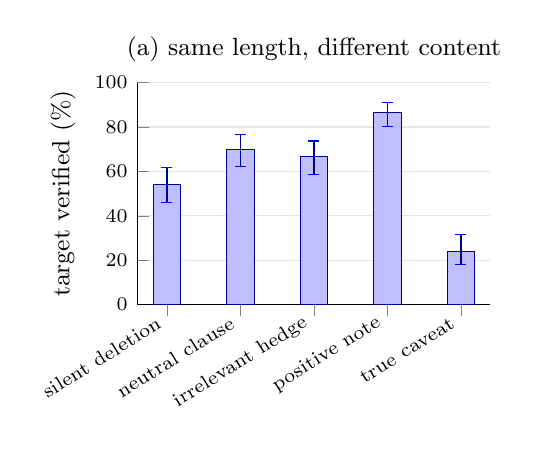
\begin{tikzpicture}
\begin{axis}[
  width=0.50\textwidth, height=4.4cm,
  ybar, bar width=10pt, ymin=0, ymax=100,
  symbolic x coords={silent deletion,neutral clause,irrelevant hedge,positive note,true caveat},
  xtick=data, x tick label style={rotate=32,anchor=east,font=\scriptsize},
  ylabel={target verified (\%)}, ylabel style={font=\small},
  tick label style={font=\scriptsize},
  ymajorgrids, grid style={gray!20}, axis lines*=left,
  title={\small (a) same length, different content}, title style={yshift=-2pt},
]
\addplot+[fill=blue!25,draw=blue!60!black,
  error bars/.cd,y dir=both,y explicit,
  error bar style={line width=0.5pt},error mark options={rotate=90,mark size=2pt}]
  coordinates {\EightArmCoords};
\end{axis}
\end{tikzpicture}
&
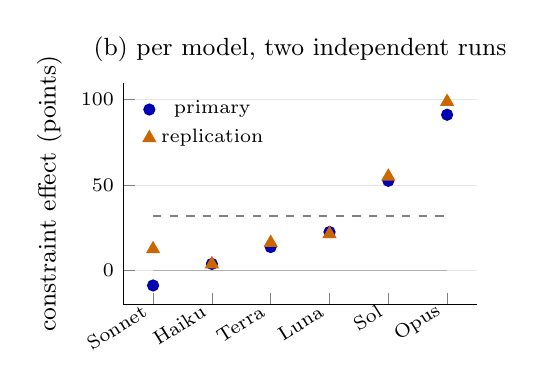
\begin{tikzpicture}
\begin{axis}[
  width=0.50\textwidth, height=4.4cm,
  ymin=-20, ymax=110,
  symbolic x coords={Sonnet,Haiku,Terra,Luna,Sol,Opus},
  xtick=data, x tick label style={rotate=32,anchor=east,font=\scriptsize},
  ylabel={constraint effect (points)}, ylabel style={font=\small},
  tick label style={font=\scriptsize},
  ymajorgrids, grid style={gray!20}, axis lines*=left,
  legend style={font=\scriptsize,at={(0.03,0.97)},anchor=north west,draw=none,fill=none},
  title={\small (b) per model, two independent runs}, title style={yshift=-2pt},
]
\addplot[only marks,mark=*,mark size=2pt,blue!70!black] coordinates {\TenModelPrimaryCoords};
\addlegendentry{primary}
\addplot[only marks,mark=triangle*,mark size=2.6pt,orange!80!black] coordinates {\TenModelReplCoords};
\addlegendentry{replication}
\draw[dashed,gray] (axis cs:Sonnet,\TenPooledLine) -- (axis cs:Opus,\TenPooledLine);
\draw[gray!60] (axis cs:Sonnet,0) -- (axis cs:Opus,0);
\end{axis}
\end{tikzpicture}
\end{tabular}
\caption{\textbf{(a)} Experiment 8, \EightN{} episodes. Four arms append a
clause of \EightAppendMin--\EightAppendMax{} characters; \emph{silent
deletion} appends none. An irrelevant hedge sits on the neutral clause
(\EightHedgeVsPadded{} points, $p = \EightHedgeVsPaddedP$): the earlier hedging
interpretation does not survive its own length control. The true caveat is
\EightCaveatVsPadded{} points below that neutral clause. Wilson 95\% intervals.
\textbf{(b)} Experiment 10 constraint effect per model, primary run and
pre-registered replication, over \TenContrastN{} episodes; dashed line the
pooled estimate (\TenPooled), solid line zero. Positive in \TenPosPrimary{} of
\TenModels{} models primary and \TenPosRepl{} of \TenModels{} replicated;
\TenFlippedModel{} is the only sign difference between runs and the least
stable model under repeated identical prompts.}
\label{fig:resolved}
\end{figure}

\section{Does what gets verified matter later?}\label{sec:downstream}

Allocation only matters if the record the budget failed to recover changes what
the agent later does. We test that directly by randomising it. A second agent
inherits the same situation together with a carried set of provenance records,
and which records are carried is assigned at random rather than chosen by the
first agent. This breaks the dependence between what an agent wanted to check
and what it ends up holding.

Carrying the source record for the corrupted memory moves the rate at which the
later decision goes in the corrupted direction from \ThreeBOthK/\ThreeBOthN{}
to \ThreeBTgtK/\ThreeBTgtN{}, and unguarded commitment --- committing without
naming the constraint --- from \ThreeBNGOth{} to \ThreeBNGTgt{}
($\ThreeBCMH$, all \ThreeBAllModels{} models in the same direction). A randomised-instrument replay --- re-running only the second decision as a
fresh session, with recovered records reproduced from each stored episode ---
agrees with the direct estimate within a point; we report it as convergent
evidence only, since the exclusion restriction it needs is untestable here.

This identifies the \emph{downstream} half of the chain: what provenance the
agent holds causally changes the decision it reaches. Together with
\S\ref{sec:directs}, which identifies the upstream half, the two halves are
established separately. We do not claim an identified end-to-end mediation from
working plan through verification allocation to later harm; no single design
here carries that, and combining two separately identified halves is not the
same as identifying the chain. Nor do we present this as the novel mechanism:
inserting the decisive contradicting record into an agent's context and
watching the decision change is close to what one would expect. Its role is to
establish that the allocation studied upstream has operational consequence.

\section{Threat-model boundary: what consolidation actually removed}\label{sec:boundary}

The controlled experiments above install the corruption by hand, deleting a
negative caveat entirely. Whether that omission arises on its own is a separate
question, and the answer bounds everything else in this paper.

\paragraph{Four things a memory can lose.} These come apart in what follows and
are not interchangeable. A \textbf{negative outcome} is an adverse empirical
result, here retention $-12$pp. A \textbf{scope constraint} restricts the
population, period or context a result holds for. A \textbf{prohibition} is a
normative instruction, ``do not reuse this''. \textbf{Complete negative
deletion} is the corruption our controlled sections install: no adverse outcome
and no warning of any kind remains.

Figure~\ref{fig:erosion} summarises what happened. We ran a benign consolidation pipeline --- \FiveChains{} chains,
\FiveGenerations{} generations, each generation asked only to compress and carry
forward, with no instruction about caveats or qualifiers --- and scored every
generation of every chain with a frozen model scorer. On the two records that
carry no qualifier in their source it returns \FiveFalsePosAll{} false
positives, and on the four that do it recovers the qualifier in
\FiveScorerSensK/\FiveScorerSensN{} first-generation bodies. Two limitations
follow it into every number below: the scorer is \texttt{\FiveScorerModel},
which is \textbf{also one of the six consolidator models}, so it is not
independent of the systems it judges; and no human validation was performed.
Its sensitivity is validated only on first-generation bodies, which are
near-verbatim; nothing validates it on the compressed final-generation bodies
where the erosion is claimed, so part of the decline could be scorer failure on
telegraphic text rather than loss of the qualifier. The negative-outcome
counts, by contrast, are deterministic keyword detection and do not depend on
the scorer at all --- and they are immune to this confound.

\paragraph{What survived.} \textbf{Complete negative deletion} appears in
\FivePurelyPositive{} chain-generations. This is the only claim the
\FivePurelyPositive{} figure supports; it is not a claim that nothing eroded. The quantified negative is durable: it is present in
\FiveNumAllGens{} chains at \emph{every} one of the six generations
(\FiveNumSeries\%), and of the \NineBodies{} distinct final-generation bodies,
\NineKeepNeg{} carry a number attached to a negative outcome or a churn or
retention term. Appendix~\ref{app:consolidation} prints final-generation bodies
verbatim, selected by a stated deterministic rule.

\paragraph{What did not.} The same scorer shows the qualifier eroding
\emph{monotonically inside the horizon we tested}. For the target memory the
share of chains still stating its qualifier runs
\FiveTgtSeries\% across the six generations, ending at
\FiveTgtGenSixK/\FiveTgtGenSixN. For the three memories whose qualifier is a scope
restriction rather than a number, it runs \FiveScopeSeries\%, ending at
\FiveScopeGenSixK/\FiveScopeGenSixN. The explicit prohibition falls too, from
\FiveProGenOneK/\FiveProGenN{} chains to \FiveProGenSixK/\FiveProGenN{}
(\FiveProSeries\%), though not monotonically, so we report the level rather
than a trend. Consolidation did not remove the number; the scope
declined monotonically and roughly half the prohibitions were gone by the sixth
generation.

\paragraph{What that does to the risky action.} Running the allocation protocol
on the final-generation bodies, a consolidated body suppresses the risky action
as completely as the intact original: it is planned in
\NineNatIntentK/\NineNatIntentN{} episodes against
\NineIntactIntentK/\NineIntactIntentN{} for the intact original and
\NineHandIntentK/\NineHandIntentN{} for the hand-stripped body. It is verified far less often than our hand-built corruption. The
prospectively specified primary contrast --- the consolidated body padded to the
hand-built body's length, because \S\ref{sec:content} shows a
\EightLengthEffect-point silent-deletion versus neutral-clause gap --- is
\NinePadVsHand{} points; unpadded, the raw gap is \NineNatVsHand{} points
(\NineNatPct\% against \NineHandPct\%). Against the intact original it is
\NineNatVsIntact{} points, a difference we do not interpret: it is smaller than
the run-to-run variability we measure in \S\ref{sec:limits} and has not been
replicated (full arm table in Appendix~\ref{app:models}). \textbf{We cannot say whether a consolidated body is harder or
easier to catch than the record it came from}; what we can say is that it is
not the corruption our controlled sections install.

\begin{center}\itshape
The allocation dependence is real, but whether it becomes harmful depends on
what memory degradation actually removes. In the benign consolidation process we
tested, the quantified negative survived all six generations and complete deletion
did not occur --- while scope fell to \FiveScopeGenSixPct\% and roughly half
the explicit prohibitions were gone.
\end{center}

\noindent We do not generalise this beyond the tested scenario, models,
consolidation procedure and \FiveGenerations{}-generation horizon, and the
erosion trend is a reason not to: it is a decline observed \emph{within} the
horizon, not a plateau. A longer horizon, a lossier or adversarial pipeline, or
a constraint expressed only as scope may well produce the omission this pipeline
did not.

\begin{figure}[t]
\centering
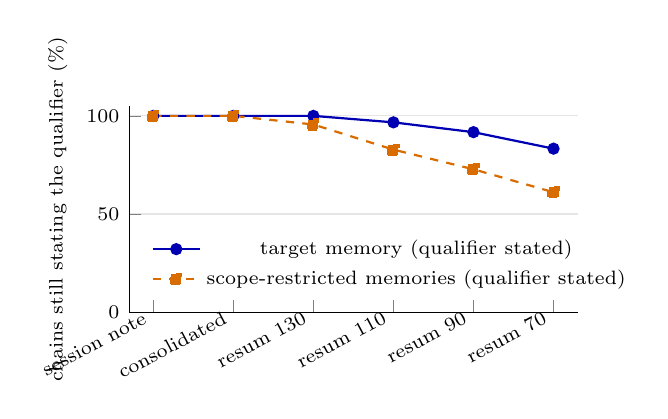
\begin{tikzpicture}
\begin{axis}[
  width=0.60\textwidth, height=4.2cm,
  xmin=0.7, xmax=6.3, ymin=0, ymax=105,
  xtick={1,2,3,4,5,6},
  xticklabels={session note,consolidated,resum 130,resum 110,resum 90,resum 70},
  x tick label style={rotate=28,anchor=east,font=\scriptsize},
  ylabel={chains still stating the qualifier (\%)}, ylabel style={font=\scriptsize},
  tick label style={font=\scriptsize},
  ymajorgrids, grid style={gray!20}, axis lines*=left,
  legend style={font=\scriptsize,at={(0.03,0.06)},anchor=south west,draw=none,fill=none},
]
\addplot[mark=*,mark size=1.8pt,blue!70!black,thick] coordinates {\FiveErosionCoords};
\addlegendentry{target memory (qualifier stated)}
\addplot[mark=square*,mark size=1.8pt,orange!85!black,thick,dashed] coordinates {\FiveScopeErosionCoords};
\addlegendentry{scope-restricted memories (qualifier stated)}
\end{axis}
\end{tikzpicture}
\caption{What six generations of benign consolidation removed, judged by a
frozen model scorer (\FiveScorerModel, itself one of the six consolidator
models) with \FiveFalsePosAll{} false positives on records carrying no
qualifier. The corruption our controlled sections install --- a body with no
negative content left --- never occurs (\FivePurelyPositive{} chain-generations).
Plotted is the scorer's judgment that the body still \emph{states} its
qualifier; the quantified negative itself never falls (\FiveNumAllGens{} at
every generation). What erodes monotonically \emph{within} the tested horizon
is the qualifier as stated: the target memory falls to
\FiveTgtGenSixK/\FiveTgtGenSixN{} and scope restrictions to
\FiveScopeGenSixK/\FiveScopeGenSixN. This is a decline observed inside the
tested range, not a plateau, and it is why we do not extrapolate the negative
result to longer horizons.}
\label{fig:erosion}
\end{figure}

\section{Discussion}\label{sec:discussion}

The results separate two questions that current memory architectures answer with
one mechanism. A retriever answers \emph{what is relevant to the present
context?} Under a verification budget the agent must also answer \emph{which
inherited belief is most costly to leave unverified?} These need not induce the same ranking. \S\ref{sec:directs} shows the agent's scarce checking follows the
first question --- attention goes where the plan already points --- and
\S\ref{sec:content} shows the second also depends on the memory's own content:
a belief that states its constraint is checked substantially less often than a
length-matched belief that does not. We
note what this does \emph{not} show: no arm in any experiment states a
constraint that is false or stale, so whether a confidently-stated but outdated
constraint escapes checking --- the case the safety motivation turns on ---
remains untested.

Nothing here shows that the allocation we measure is \emph{wrong}. Every
constraint in every arm of every experiment is true, and declining to spend a
scarce credit re-deriving a true, already-stated constraint is locally sensible.
The concern is narrower and conditional: \emph{if} present relevance and future
expected loss diverge, a policy dominated by the former could under-check
beliefs whose later staleness would be costly. We do not establish that this
occurs. Testing it requires a constraint that is false or out of date, which we
do not run.

With that bound stated, verification scheduling is worth separating from
retrieval and from provenance storage as a control layer with its own inputs: relevance to the current plan,
loss if the belief is wrong, how many consolidation steps the record has passed
through, how far its scope has broadened, and when it was last checked. We do
not evaluate such a scheduler, and we could not identify a normatively correct
verification order from this data: that would require a corruption prior, a
distribution over future contexts and a loss model, none of which these
experiments supply. The contribution is the measurement that motivates building
one.

\section{Limitations}\label{sec:limits}

\textbf{Stochastic instability at the episode level.} Re-running
\StabilityN{} byte-identical prompts flips \StabilityFlip{} outcomes
(\StabilityFlipPct\%), ranging from \StabilityMin\% to \StabilityMax\% by model,
with \StabilityWorstModel{} least stable. Small effects here require replication before they are interpreted; that is why \S\ref{sec:content} reports primary and replication runs, and why we do not interpret contrasts of a few points.

\textbf{Model heterogeneity.} Magnitudes vary by an order of magnitude across
models (\S\ref{sec:content}). We avoid claims about language models in general.

\textbf{Geometry and scenarios.} Six inherited memories and a budget of one to
three is small against a production store, and the scenarios are synthetic. The allocation signature was reproduced across \SixModels{} models in two
worlds beyond the one the mechanism experiments use, but those mechanism
experiments use a single world.

\textbf{Prompting and structured output.} All results are obtained through a
fixed system prompt and a strict JSON schema. \S\ref{sec:directs} shows the main
causal result strengthens when the action field is removed, but the protocol is
not the only way to elicit these behaviours.

\textbf{The plan manipulation bundles three things.} \S\ref{sec:directs}
cannot separate working-plan state from the topical salience of naming the plan
or from directive framing. The randomised intervention effect stands; its
internal composition is not identified, and the discriminating cell was not
run.

\textbf{What is not identified.} The upstream and downstream halves of the chain
are identified separately and not end to end. Intent is measured after treatment
and is a candidate mediator; we compute no contrast on it and claim no
mediation. \S\ref{sec:content} does not identify a causal main effect of
register.

\textbf{Adaptive history.} Several interpretations reported in earlier versions
of this work were falsified by our own pre-registered tests and have been
withdrawn: the hedging effect of \S\ref{sec:content}, and the claim that
naturally consolidated records are harder to catch than the record they came
from. Pre-registrations, amendments and every episode file are in the
supplementary record.


\paragraph{Data and code availability.} Pre-registrations, amendments, analysis
scripts and every episode file are archived in the supplementary material;
every printed number regenerates from them.

\bibliography{refs-full}

\appendix
\section{Per-model results}\label{app:models}

\paragraph{Experiment 7 (plan assignment, verify-only).} Verification of the
pricing memory by assigned plan, per model; the no-plan column is the baseline
arm. $\Delta$ is pricing minus onboarding in points.

\begin{center}\small
\begin{tabular}{lcccc}
\toprule
model & pricing & onboarding & no plan & $\Delta$ \\
\midrule
\texttt{claude-haiku-4-5} & 12/25 & 0/25 & 0/25 & $+48.0$ \\
\texttt{claude-opus-5} & 25/25 & 1/25 & 25/25 & $+96.0$ \\
\texttt{claude-sonnet-5} & 25/25 & 3/25 & 25/25 & $+88.0$ \\
\texttt{gpt-5.6-luna} & 25/25 & 0/25 & 2/25 & $+100.0$ \\
\texttt{gpt-5.6-sol} & 25/25 & 5/25 & 23/25 & $+80.0$ \\
\texttt{gpt-5.6-terra} & 25/25 & 1/25 & 24/25 & $+96.0$ \\
\bottomrule
\end{tabular}

\end{center}

\paragraph{Experiment 10 (constraint effect), primary and replication.}
Removed minus retained, in points. Values are exact multiples of $1/80$
(cell sizes are 40 and 80 per model per run), rounded half away from zero, so
identical underlying rates print identically.

\begin{center}\small
\begin{tabular}{lcc}
\toprule
model & primary & replication \\
\midrule
\texttt{claude-opus-5} & $+91.3$ & $+98.8$ \\
\texttt{gpt-5.6-sol} & $+52.5$ & $+55.0$ \\
\texttt{gpt-5.6-luna} & $+22.5$ & $+21.3$ \\
\texttt{gpt-5.6-terra} & $+13.8$ & $+16.3$ \\
\texttt{claude-haiku-4-5} & $+3.8$ & $+3.8$ \\
\texttt{claude-sonnet-5} & $-8.8$ & $+12.5$ \\
\bottomrule
\end{tabular}

\end{center}

\paragraph{Experiment 9 arm table.} Body length shown, first-pass plans of the
risky action, and verification of the target.

\begin{center}\small
\begin{tabular}{lcccc}
\toprule
arm & body chars & plans risky action & verifies target & rate \\
\midrule
natural (consolidated body) & 64--134 & 0/150 & 34/150 & 22.7\% \\
natural, padded to 129 chars & 120--139 & 0/150 & 46/150 & 30.7\% \\
hand-stripped corruption & 129--129 & 28/150 & 91/150 & 60.7\% \\
intact original & 221--221 & 0/150 & 36/150 & 24.0\% \\
\bottomrule
\end{tabular}

\end{center}

\section{Episode-level stability}\label{app:stability}

The Experiment 9 sensitivity run re-issued \StabilityN{} byte-identical prompts
(the punctuation repair touched only 23 of 150 bodies, leaving the rest
unchanged), giving a direct measurement of run-to-run variability:
\StabilityFlip{} of \StabilityN{} episodes (\StabilityFlipPct\%) flip their
binary outcome, and the aggregate rate moved 6.3 points from sampling alone.

\begin{center}\small
\begin{tabular}{lcc}
\toprule
model & flips & rate \\
\midrule
\texttt{claude-haiku-4-5} & 2/23 & 8.7\% \\
\texttt{claude-opus-5} & 2/22 & 9.1\% \\
\texttt{claude-sonnet-5} & 8/19 & 42.1\% \\
\texttt{gpt-5.6-luna} & 4/22 & 18.2\% \\
\texttt{gpt-5.6-sol} & 8/21 & 38.1\% \\
\texttt{gpt-5.6-terra} & 8/20 & 40.0\% \\
\bottomrule
\end{tabular}

\end{center}

This is not a universal threshold below which effects are zero. It means that
small aggregate contrasts in this protocol require independent replication
before they are interpreted, which is why \S\ref{sec:content} reports two runs
and why the paper declines to interpret contrasts of a few points.

\section{Consolidation outputs and scorer validation}\label{app:consolidation}

\paragraph{Final-generation bodies, verbatim.} The first four of the
\NineBodies{} distinct final-generation target bodies in lexicographic order
--- a stated deterministic rule, so the examples cannot be cherry-picked:

\begin{description}\small
\item[78 ch] \texttt{40\% SMB discount: +31\% signup,+18\% rev short-term,-12\% ret. AVOID, not a lever}
\item[92 ch] \texttt{40\% SMB discount: +31\% signup,+18\% rev short-term,-12\% retain,pre-renewal churn. Avoid reuse}
\item[77 ch] \texttt{40\% SMB discount: +31\% signup,+18\% rev,-12\% ret, renewals fail. One-off only.}
\item[64 ch] \texttt{40\% SMB discount: +31\% signup/+18\% rev/-12\% retain; one-off only}

\end{description}

Compression is severe and the register is telegraphic, but the quantified
negative and, in many bodies, an explicit prohibition survive.

\paragraph{Scorer validation, both directions.} The frozen scorer is
\texttt{\FiveScorerModel}, which is also one of the six consolidator models, so
it is \emph{not} independent of the systems it judges; no human validation was
performed. On the \FiveUnqualifiedMems{} records carrying no qualifier in their
source it returns \FiveFalsePosAll{} false positives (specificity); on the
\FiveQualifiedMems{} records that do, it recovers the qualifier in
\FiveScorerSensK/\FiveScorerSensN{} first-generation bodies (sensitivity). The
quantified-negative counts in \S\ref{sec:boundary} are deterministic keyword
detection and do not depend on the scorer.

\section{Pre-registration record}\label{app:prereg}

Each confirmatory experiment's pre-registration --- hypotheses, thresholds,
exclusion rules and the analysis script --- was committed to version control
before its first model call; for the six experiments whose registration and
first episode are both timestamped, the registration precedes the first episode
file by between 9 seconds and 6 minutes. The record also contains what a
faithful history requires: the Experiments 3--5 registration carries three
amendments (two written after a pilot, before the registered run), the
Experiment 6 registration carries twenty-two, and Experiment 5b was exploratory
throughout --- its observation was later reproduced by the pre-registered
Experiment 9, which is the only sense in which it is confirmed. One registered
hypothesis (H32, Experiment 7) was breached and is reported as such in
\S\ref{sec:directs}. The registrations, amendments, analysis scripts and every
episode file (exact prompts, memory bodies, seeds, raw responses, scoring) are
in the supplementary record.

\section{Withdrawn interpretations}\label{app:falsified}

Earlier versions of this work, including a published preprint, reported
interpretations that our own later pre-registered tests falsified. They are
recorded here so that no reader reconstructs them from the earlier text.

\begin{itemize}\itemsep2pt\small
\item \emph{``Silence is stealthier than qualification''} --- an irrelevant
hedge was reported to draw more scrutiny than silent deletion. The
pre-registered length-matched control gives \EightHedgeVsPadded{} points
($p=\EightHedgeVsPaddedP$); the original gap was the \EightLengthEffect-point
silent-deletion versus neutral-clause contrast, which bundles length, clause
existence and neutral content.
\item \emph{Naturally consolidated records are stealthier than the intact
original} --- the measured difference is \NineNatVsIntact{} points, inside
run-to-run variability, never replicated, and not interpreted.
\item \emph{Telegraphic register explains the natural-versus-hand-built gap}
--- the constraint effect is positive within both registers (\TenFluent{} and
\TenTelegraphic) and the marginal register contrast is \TenSyntax{} points.
\item \emph{Unquantified claims attract checking} --- the unquantified bridge
body is verified \TenBridgeDelta{} points \emph{less} than its quantified
match; the sign is reversed.
\item \emph{Punctuation drives verification} --- re-running the same 23 bodies
with only a full stop changed moves $-8.7$ points, exact McNemar $p=0.774$.
\item \emph{Low verification because the risky action was already rejected} ---
episodes that rejected the action still verify the hand-built corruption at
51.6\%, and three models with zero intent variance show $-25.3$ points.
\item \emph{The observed policy is normatively wrong} --- every constraint in
every arm is true; the normative case (a false or stale constraint) is untested
(\S\ref{sec:discussion}).
\end{itemize}


\end{document}
